\documentclass{article}
\usepackage{graphicx} % Required for inserting images
\usepackage{listings}
\usepackage{url} % Add the url package
\usepackage{titlesec}

\documentclass{article}
\usepackage{graphicx} % Required for inserting images


\usepackage{titlesec}

\title{ECS171 Group 8 Report}
\author{Boquan Fang, Sage Deo, Ishita Dutta, Zhuo Chen}
\date{June 2023}
% \url{https://github.com/BoquanFang/ECS171_Term_Project.git}



\maketitle

\begin{document}

\section{Introduction}
Listening to music is a popular activity that people all over the world engage in. 
Everyone has their own music taste and their own way of listening to music.
Some people exclusively listen to music by picking a single album by a single artist 
and listening to it from beginning to end, but others curate playlists of music from
various albums by various artists. These playlists are often designed to suit specific
moods or feelings, and it is important to the listening experience that the contents of
each playlist is internally consistent to avoid jarring the listener or inducing whiplash.

Prior to the creation of intelligent recommender systems such as those employed by 
Spotify and YouTube Music, humans would create playlists for themselves or for others,
and thus would seleect songs for each playlist that both fit that playlist's desired mood
and are tonally similar to the other songs on the playlist. However, as such 
online music platforms emerged, they became ways of exploring new types of music cheaply.
Users did not have to spend money on physical media or digital rights to a song that they
might not enjoy, so they could listen to lots of music themselves to determine if they liked it
or not. Later, as content recommendation algorithms became stronger and amassed more data
to train on, automatic recommendation methods became a viable way for users of these platforms
to find new music to listen to without having to listen to all the songs themselves. 

Thus, the problem of this research paper is about determining whether a chosen song is similar enough to others in a given playlist to be accepted into that playlist. This can be used to recommend new songs to the user based on the contents of their existing playlists; users are more likely
to enjoy songs that can fit into their existing playlists, especially those they listen to most.
Additionally, it can be used to generate entirely new playlists for users, starting from a small
playlist of a few of their favorite songs, and then repeatedly searching for and adding songs that
fit the energy of the newly-generated playlist. This creates completely new full-sized playlists 
with consistent energy and tone and potentially new songs that the user has not listened to before.
This will create a novel but still enjoyable listening experience. 

\section{Literature Review}
Some study has been done on Spotify data. For example, Nijkamp et al. used the Spotify API
to investigate whether a song's popularity could be predicted based on its other features, and found
that it could not. Pareek et al. also found that a random forest model could classify songs
as popular or unpopular with an accuracy of 86\%. Code AI managed to predict popularity with a KNN
model with an error of only 0.03\%. However, all of these studies are addressing the problem
of predicting popularity; there is currently a gap in knowledge surrounding the problem of fitting
songs into playlists. 

One instance of using machine learning to recommend songs rather than predict their popularity is
Alexander Bricken's Gaussian Mixture model which recommend songs based on their Spotify API
features. Though this is not exactly the same as determining whether a song fits into a playlist,
it is similar and a useful starting point.

\section{Dataset Description and Exploratory Data Analysis of the Dataset}
This project’s dataset is retrieved by the user level interface from the Spotify developer API. With two given URL to a playlist and a song, the user level interface could access the Spotify developer API and save the data for both the playlist and the given song in a CSV file. The number of rows is depended on how many songs that a given playlist has. The Spotify developer API provides thirteen attributes for a given song: name, danceability, energy, key, loudness, mode, speechiness, acousticness, instrumentalness, liveness, valence, tempo, and duration. The name represents the name of a given song and that would not be considered in our exploratory data analysis part. Danceability “describes how suitable a track is for dancing based on a combination of musical elements including tempo, rhythm stability, beat strength, and overall regularity.” Energy represents “is a measure from 0.0 to 1.0 and represents a perceptual measure of intensity and activity.” Key represents the track that a given music is in. Loudness shows the overall loudness of a song in decibels.  Mode indicates “the modality (major or minor) of a track, the type of scale from which its melodic content is derived”. Speechiness indicates the presence of oral spoken words in the given song. Acousticness is the confidence interval of the track in terms of acoustic. Instrumentalness “predicts whether a track contains no vocals.” Liveness detects “the presence of an audience in the recording.” Valence is “a measure from 0.0 to 1.0 describing the musical positiveness conveyed by a track.” Temp covers “the overall estimated tempo of a track in beats per minute (BPM).” The attributes duration indicates the duration of the songs in millisecond. 
The attributes energy is the most important attribute, since we will use the energy attribute as an indicator of whether the given song fits well with the playlist. Therefore, exploratory analysis needs to generate a correlation heat and analyze the correlation between every attribute with respect to the energy attribute. The group determines that every attribute which has a correlation that less than 0.2 in absolute value should not be included in the final training set. If those attributes are included in the training set, those attributes will generate noise and overfit the model.

\section{Proposed Methodology}
To go about determining whether a song would match the energy of a playlist, we decided to do the following steps:
1. Run the Spotify API in order to get the information for the input playlist and later the song inputted into test the fit for the energy of the playlist.
2. Preprocess our training set, or the given dataset of our playlist so that we were able to get a more standard method of measurement. 
3. Run the model and determine an energy category prediction for the new playlist
4. Determine a conclusion based on the standard determination of the songs in the playlist.

To complete the first step, we visited the spotify for developers website [1]. In this, we were able to create a login key that would allow us to run the API for gathering song data. Here, we decided to parse the URL for the specific guid that would identify the public playlist. After a few more parameters, we were able to get our data and display it on our interface, as well as save the data to a file called `songs.csv`. We also did the same for the new song and saved that to a file called `rand_song.csv`.

From here, we starting focusing on the model and specifications necessary for running the model properly. To do this while we were stilly figuring out the API, we decided to use a practice dataset from Kaggle [2]. Using this set covering the same variables over 20.0k songs, we learned more about the measures and what preprocessing steps we should take in order to have a standard model.

For preprocessing our data, we decided to place all of our energy levels into a category called `energy_categories`. What this did was create the buckets for the classification algorithms to predict the new song's energy level. To do this, we took the original energy between the interval  [0.0, 1.0] and floor divided by 0.01 to have a maximum of 100 energy categories. We chose 0.01 for the most accuracy while still keeping the differences of the dataset and to make all the numbers integers (avoiding 0.5 values) to better classify into buckets. This helped create a more feasible output for the model, while still keeping the values as accurate as possible. We then made a histogram showing the distribution of the `energy_category` values. Here, we realized that, due to the law of large numbers, we would not need to worry too much about the normality of the data and carried on with the data normality assumption. This was due to observing not only the Kaggle dataset, but multiple playlists pulled from the spotify interface, all showing similar to bell curve histograms

We then dropped the `Name` variable for having a more blind analysis, so that the model would not confuse the `Name` as one of the evaluatory measures and skew the ouptut. From here, we decided to 
create the correlation heatmap of our data, so that we could determine the necessary variables for a more accurate analysis. We decided to do this for two endpoint reasons. The first reason was that we did not want to include all of the variables in our analysis. Some of the variables like `Mode` and `Instrumentalness` were displaying really low correlations to the energy with our Kaggle dataset. Including these variables meant that we were introducing more noise to our model rather than giving it data to make a more accurate analysis. The second was to determine a sort of pattern that would tell us how to determine which variables were best for our model. To elaborate, we found that some variables correlate more than others when the playlist would change. Because of the lack of a static training set, we had to set preprocessing patterns such that we would be able to handle any given playlist. This meant that we would use a threshold for the correlation to the original `Energy` variable so that we would be able to accommodate for all different correlation patterns. We chose the threshold 0.2 because we saw that for most data, we would have more than 2 variables for our X when we would have the threshold, so that became our sweet spot. A higher threshold meant we were not getting the necessary amount of variables for an accurate prediction, while the lower threshold meant having too much noise. 

After removing the unneccessary variables using a more dynamic code, we decided to plot the heatmap again to check that all the necessary variables were still in the dataset, and display which variabls are being used. From there we ran our model.

We chose two proposed methodologies when working on determining our conclusion. 
One of the methodologies was running a polynomial regression model on our data.
The polynomial regression model is a model that follows a regression sense, in which each variable is assigned a constant to be multiplied to, so following the:

The other method proposed was running a KNN model [3]. Described more in the source, this model is essentially classifying a new point based on the information from the training set for a certain number of neighbors. If this means that the number of neighbors is from category A, then the model will classify A, whereas if the neighbors are category B, then classify category B. This is classified using the euclidian distance of the points as a vector(ie. each of the songs is a seperate vector of all the x variables) For this model, we decided to keep our model as dynamic as possible and started looking at ways we could determine the k number of neighbors needed for the model. We decided on a sqrt(n) [4] neighbors. Essentially, this means if we have 100 songs in our playlist, the model looks at the 10 nearest neighbors (but if the playlist number is something like 90, or a number between 2 perfect squares, it will round using the 0.5 rule).

\section{Experimental Results}

\section{Interface Design}
\maketitle
\subsection{Interface Introduction}
Once we have developed the model, we should use Flask to create an API that allows users to input a playlist and get the desired results. Flask is a popular Python web framework that is suitable for building lightweight web applications and APIs.
\begin{lstlisting}[language=Python]
# You can use this command to install the flask
pip install flask
\end{lstlisting}


\subsection{User Interface}
To create a website using Flask that allows users to input a playlist URL and extract its attributes, you'll need to perform the following steps:
1. Get an access token for the Spotify Web API:
You should first Register a new application on the Spotify Developer Dashboard (https://developer.spotify.com/dashboard/applications).
Obtain the client ID and client secret and then get the access token.
2. Use the access token to get the playlist data.
3. Get the song names and audio features from the playlist data
4. Creating a text box for a user to enter a single song's URL and retrieve its data.
5. Run the model on the page that we open, and get all the results based on our training model(the Traning dataset is the whole playlist, the test dataset is the song that we enter.


\subsection{API: Get the song names and audio features from the playlist data}
You should first make a get request to the API URL. Then, parse the response to retrieve the relevant information. The response will include an array of track objects, each containing various details about the track. I will show the code below since this part might be difficult to understand.
\begin{lstlisting}[language=Python]
# Python code snippet
    api_url = f'https://api.spotify.com/v1/playlists/{playlist_id}/tracks'
    headers = {'Authorization': f'Bearer {access_token}'}
    response = requests.get(api_url, headers=headers)
    response_data = response.json()

    # Get the song names and audio features from the playlist data
    song_names = []
    audio_features = []
    sp = spotipy.Spotify(auth=access_token)
    for item in response_data['items']:
        track_uri = item['track']['uri']
        track_name = item['track']['name']
        song_names.append(track_name)
        audio_features.append(sp.audio_features(track_uri)[0])

\end{lstlisting}
To accomplish the tasks you mentioned, we need to create four HTML files: index.html, music.html, song.html, and songs.html.

index.html: This file will serve as the welcome page where users can enter the playlist URL. It should contain necessary HTML elements such as input fields, buttons, and a form to gather user input.

music.html: This file will include essential code for integrating with the Spotify API or any other music-related functionality you're implementing. 

songs.html: This file is essential for displaying song attributes and allowing users to select a single song as a test case. It should include HTML elements to show song details such as title, artist, album, and other relevant information.

song.html: This file will display detailed information about a single song, including its attributes and several graphs to support your model. Additionally, it can include the final test result to assess the performance of your model. It uses HTML elements like headings, paragraphs, charts, or visualizations to present the information effectively.
% \subsection{Figure 1}
\begin{figure}[h]
\centering
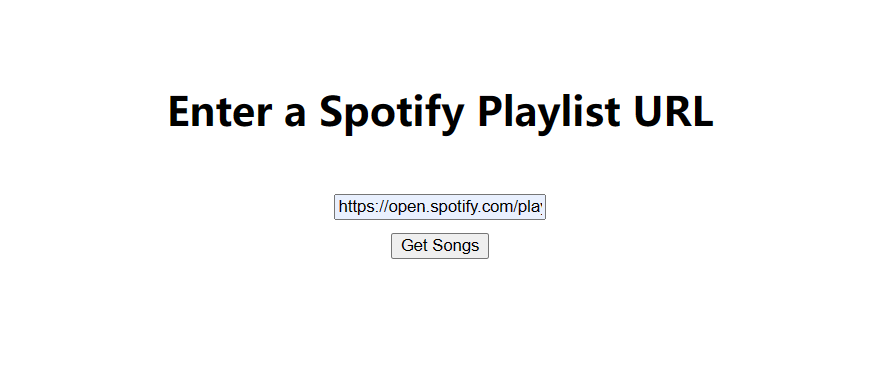
\includegraphics[width=1\textwidth]{1.png}
\caption{This is the welcome page of the user interface}
The user could enter any playlist URL here.
\label{fig:enter-label}
\end{figure}
\begin{figure}[h]
\centering
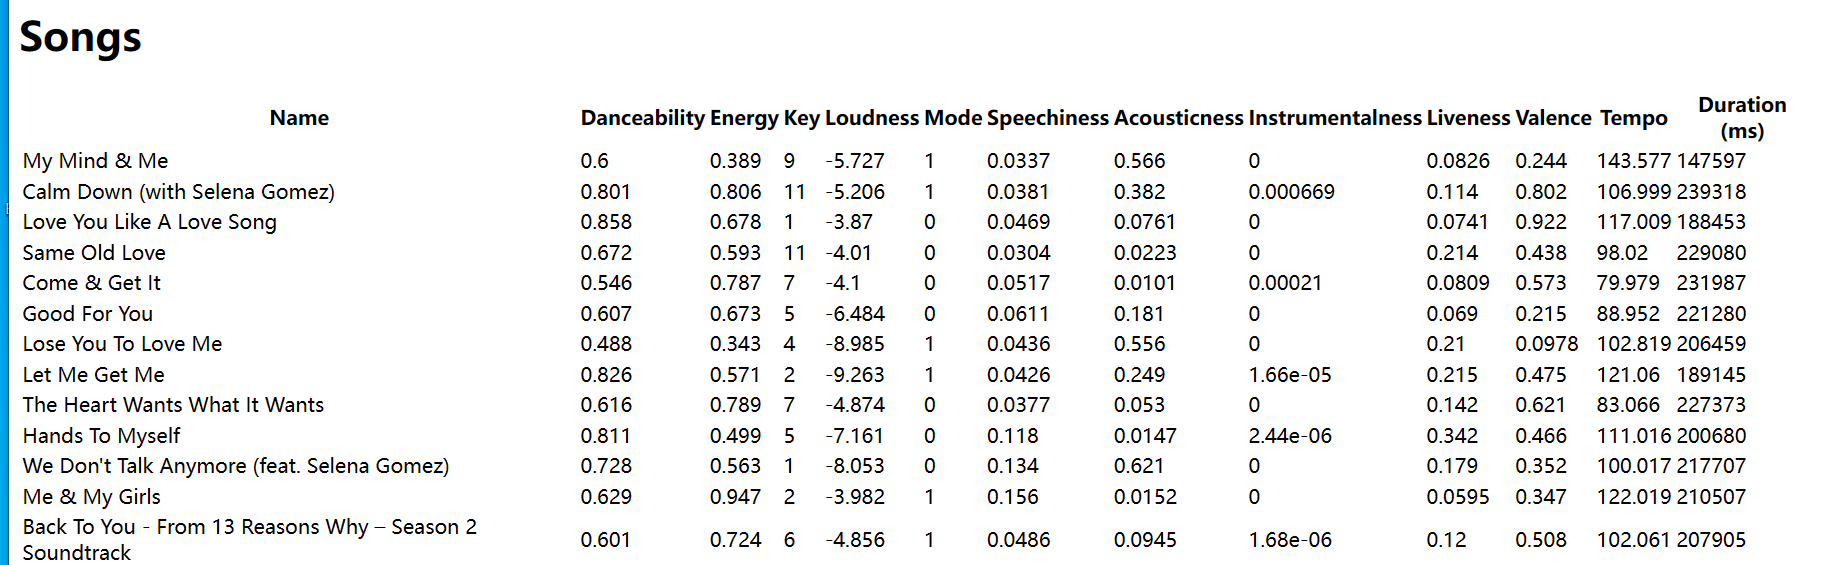
\includegraphics[width=1\textwidth]{2.png}
\caption{This is the attribute that we extract from the playlist.}
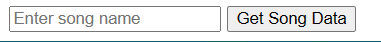
\includegraphics[width=0.5\textwidth]{3.png}
\caption{The user can enter any song's URL as the test dataset here.}
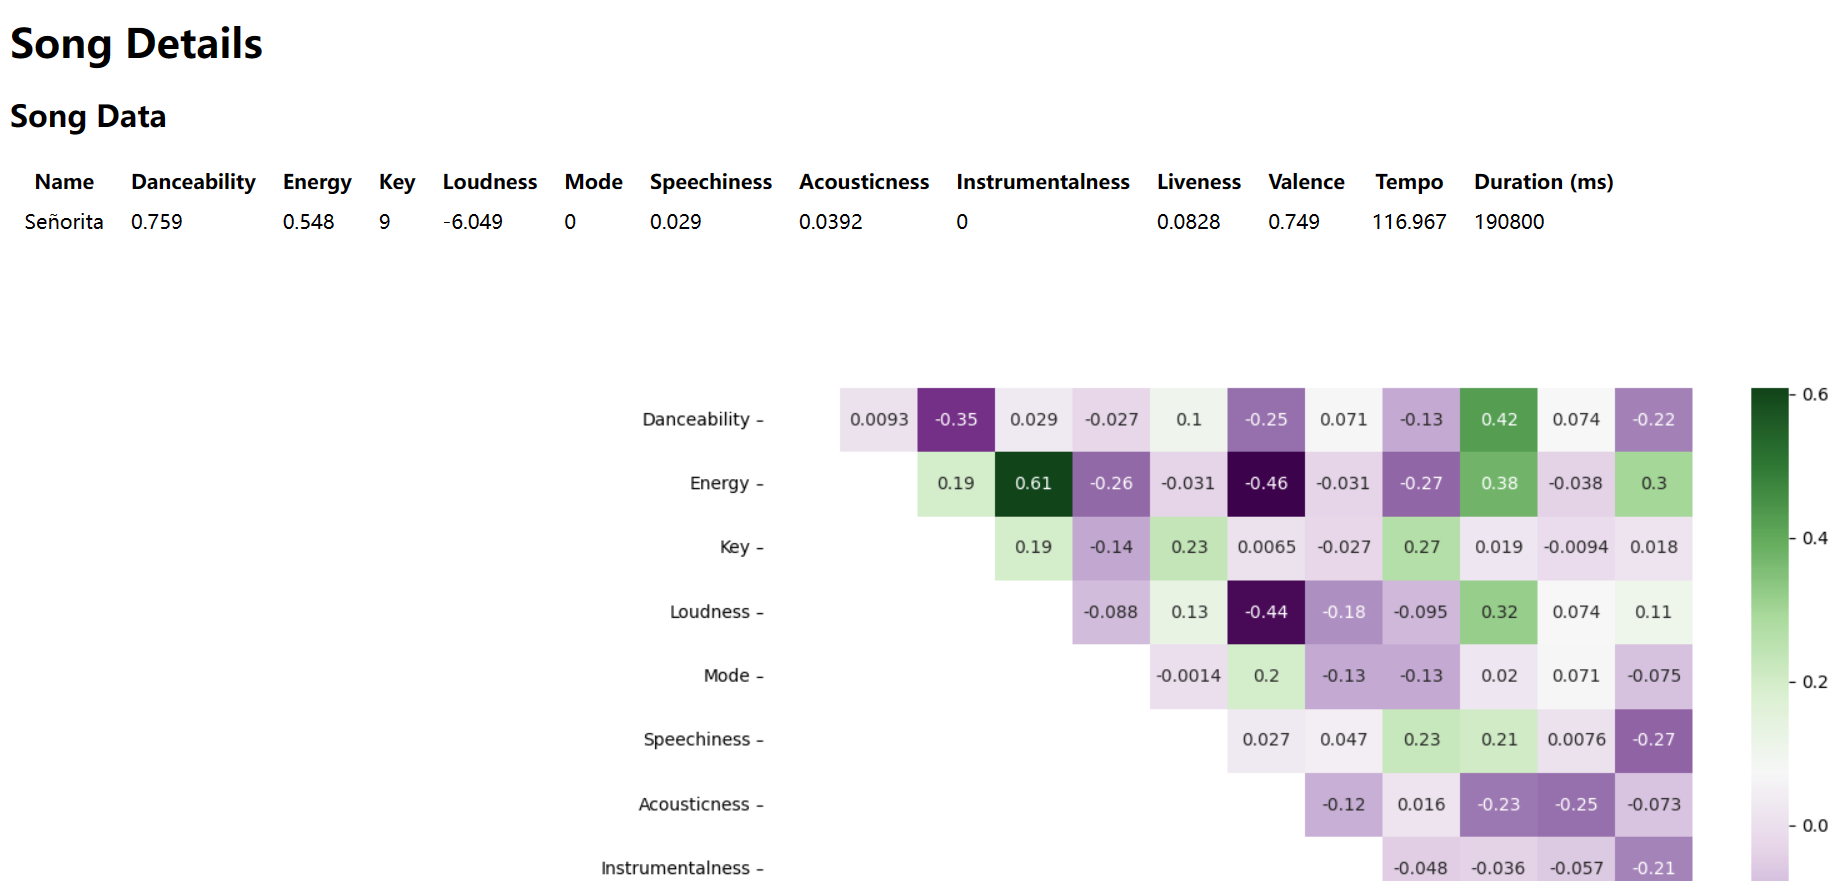
\includegraphics[width=1\textwidth]{4.png}
\caption{Here is a new page after the user enters the song's URL, and we can see the attributes of this song.}
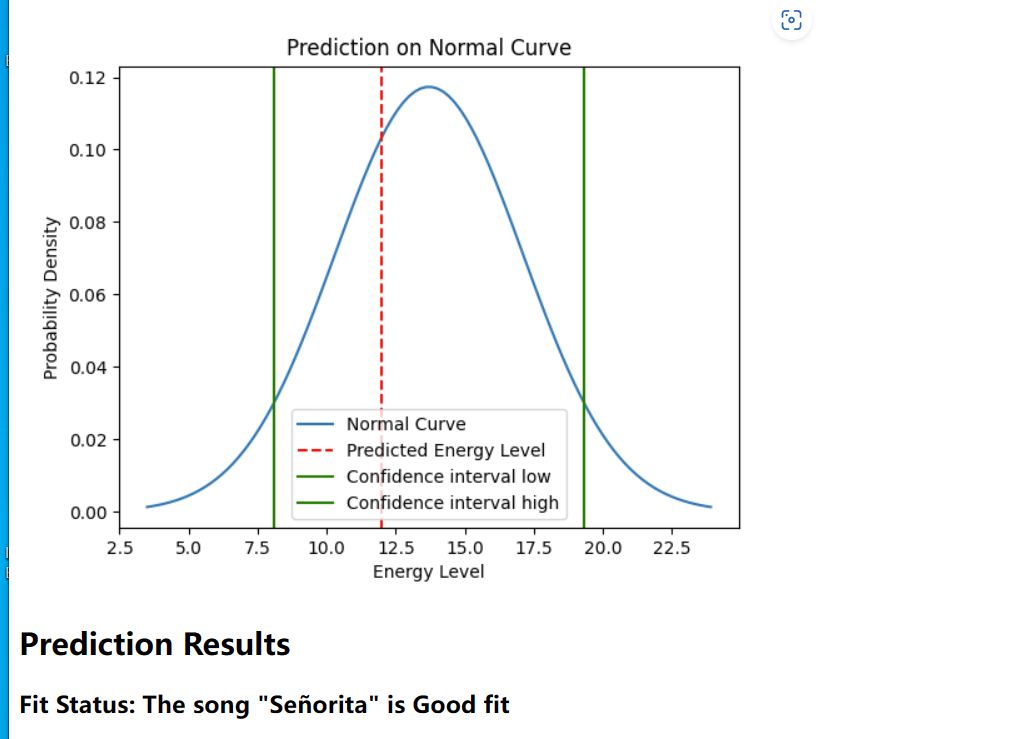
\includegraphics[width=1\textwidth]{5.png}
\caption{Finally, it shows the result at the bottom of the page about whether this song's style is similar to our playlist.}
\label{fig:enter-label}
\end{figure}
\clearpage

\section{Conclusion and Discussion}
The accuracy of the project can be further improved by incooperating different methods to get an optimal models. For example, we can
ask the user to input a playlist with at least 75 songs. The larger the dataset is, the better it will get trained. Furthermore, we
can also include k-fold validation in order to get the optimal model. 

We can also use more than just the energy attribute to be our predicted criteria. The model will predict the result better if it is not
simply rely on the entergy level. The model could include loudness into the predicted value, since loudness is another main reason people
put a song into the given playlist.

This model can be futher developed into other recommending system such as TV shows, or movie recommendation with proper input. 


\end{document}
